% CVPR 2023 Paper Template
% based on the CVPR template provided by Ming-Ming Cheng (https://github.com/MCG-NKU/CVPR_Template)
% modified and extended by Stefan Roth (stefan.roth@NOSPAMtu-darmstadt.de)

\documentclass[10pt,twocolumn,letterpaper]{article}

%%%%%%%%% PAPER TYPE  - PLEASE UPDATE FOR FINAL VERSION
%\usepackage[review]{cvpr}      % To produce the REVIEW version
\usepackage{cvpr}              % To produce the CAMERA-READY version
%\usepackage[pagenumbers]{cvpr} % To force page numbers, e.g. for an arXiv version

% Include other packages here, before hyperref.
\usepackage{graphicx}
\usepackage{amsmath}
\usepackage{amssymb}
\usepackage{booktabs}
\usepackage{listings}
% It is strongly recommended to use hyperref, especially for the review version.
% hyperref with option pagebackref eases the reviewers' job.
% Please disable hyperref *only* if you encounter grave issues, e.g. with the
% file validation for the camera-ready version.
%
% If you comment hyperref and then uncomment it, you should delete
% ReviewTempalte.aux before re-running LaTeX.
% (Or just hit 'q' on the first LaTeX run, let it finish, and you
%  should be clear).
\usepackage[pagebackref,breaklinks,colorlinks]{hyperref}


% Support for easy cross-referencing
\usepackage[capitalize]{cleveref}
\crefname{section}{Sec.}{Secs.}
\Crefname{section}{Section}{Sections}
\Crefname{table}{Table}{Tables}
\crefname{table}{Tab.}{Tabs.}
\lstset{
	basicstyle=\fontsize{8}{10}\selectfont\ttfamily
}
\graphicspath{{images}}

%%%%%%%%% PAPER ID  - PLEASE UPDATE
\def\cvprPaperID{*****} % *** Enter the CVPR Paper ID here
\def\confName{CVPR}
\def\confYear{2023}


\begin{document}

%%%%%%%%% TITLE - PLEASE UPDATE
\title{Deep Learning Fundamentals\\
	Assignment 1 - Predicting Diabetes: Perceptron Method}

\author{Ziyang Ye\\
The University of Adelaide\\
{\tt\small a1707805@adelaide.edu.au}}
\maketitle

%%%%%%%%% ABSTRACT
\begin{abstract}
	Diabetes is a chronic disease that can cause serious complications. Machine Learning can identify patterns in large amounts of data and make predictions based on those patterns.
	Perceptron, as a binary linear classifier, can predict whether a patient has diabetes based on patient-related information.
	Therefore, in the diagnosis of diabetes, the algorithm should be able to predict whether a patient has diabetes based on the patient's relevant information, such as age, gender, weight, diet, exercise, and blood sugar levels.
	This short paper describes its principles, implementation, and evaluation.
\end{abstract}

%%%%%%%%% BODY TEXT
\section{Introduction}
\label{sec:intro}

Due to the development and growth of Artificial Intelligence (AI) technology and medical data, Machine Learning (ML) algorithms are widely applied in the medical field.
The most common scenario is disease diagnosis. \\
\indent Perceptron, a classic binary classification machine learning algorithm, draws inspiration from the functioning of biological neurons, and in the field of artificial neural networks, it is also referred to as a dense (linear) layer neural network.
Perceptron can predict whether a patient has diabetes based on patient-related information such as age, gender, weight, diet, exercise, and blood sugar levels. \\
\indent In this short paper, I will explore the application of the Perceptron algorithm in diabetes diagnosis.
This paper includes the principles, implementation, and evaluation of the perceptron on the diabetes dataset.
In addition, in order to better understand the Perceptron, it is necessary to add some other methods in the experiment section.
By understanding the limitations of the Perceptron, we can better understand a series of machine learning algorithms.

\section{Related Work}
\label{sec:related}

\noindent\textbf{Logistic Regression} is a probabilistic classification model that uses the logistic function (Sigmoid function) to map the linear combination of input features to probability values between $[0, 1]$.
It outputs a probability, indicating the likelihood of belonging to the positive class\cite{wright1995logistic}. \\
\indent In other words, logistic regression uses the Sigmoid function as its activation function and binary cross-entropy (BCE) as its loss function.
\begin{equation*}\label{eq:logistic}
	\begin{gathered}
		z = \theta^{T}{x}+b \\
		g(z) = \frac{1}{1+e^{-z}} \\
		H(x) = g(\theta^{T}{x}) = \frac{1}{1+e^{-(\theta^{T}{x}+b)}} \\
		L(\theta,b) = \sum^{m}_{i=1}y_{i}\log({H(x_{i})})+(1-y_{i})\log(1-H(x_i)) \\
		J(\theta,b) = -\frac{1}{m}\sum^{m}_{i=1}y_{i}\log({H(x_{i})})+(1-y_{i})\log(1-H(x_i))
	\end{gathered}
\end{equation*}
where $\theta$ is weights, $x$ is input features, $g(z)$ is the Sigmoid function, $H(x)$ represents the logistic regression itself, $L(\theta,b)$ is the log-likelihood function and $J(\theta,b)$ is the loss function.\\
\begin{figure}[t]
	\centering
	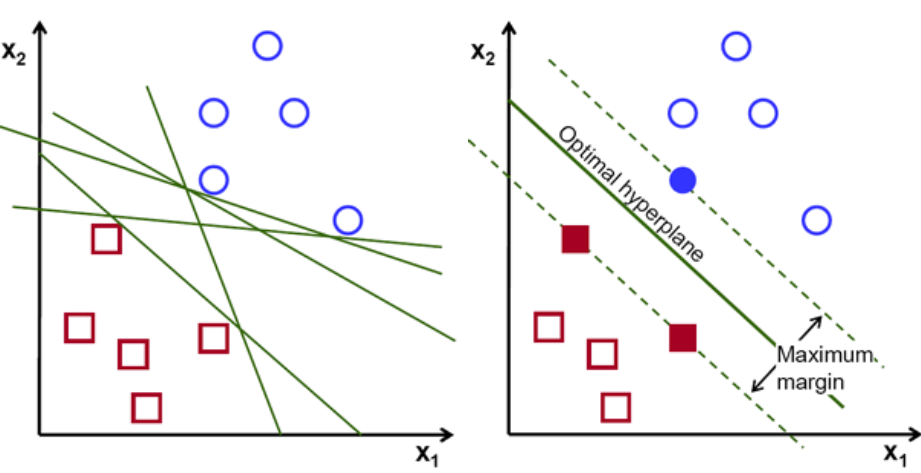
\includegraphics[width=\columnwidth]{svm-lr}
	\caption{Right is a classic linear classifier, left is SVM with hard-margin}
	\label{fig:svm-lr}
\end{figure}
\noindent\textbf{Support Vector Machine} (SVM) and perceptron are both used for classification, and they both use the sign function as the decision function. SVM optimizes its parameters by maximizing the minimum distance of support vectors from the hyperplane\cite{suthaharan2016support}.\\
\indent SVM can address both linearly separable and non-linearly separable problems using hard-margin, soft-margin, and kernel methods. It can also be transformed into a dual form using Lagrange multipliers to enhance efficiency and subsequently introduce kernel methods\cite{suthaharan2016support}.\\
\\
\noindent\textbf{Multi-Layer Perceptron} (MLP) \wrt Feedforward Neural Network, is an extension of the single-layer Perceptron and is a typical deep learning model. Its main feature is having multiple layers of neurons. Typically, the first layer of the MLP is referred to as the input layer, the intermediate layers are called hidden layers, and the final layer is the output layer. The key to using the MLP lies in training the connection weights between the layers using the backpropagation\cite{werbos1990backpropagation} (BP) algorithm, and it employs nonlinear activation functions \eg Rectified Linear Unit\cite{glorot2011deep} (ReLU) (since Sigmoid has a high computational cost).
\indent MLP does not specify the number of hidden layers, so you can choose an appropriate number of hidden layers based on your specific processing requirements. There are also no restrictions on the number of neurons in each layer of the hidden and output layers. Through hidden neurons, complex interactions between inputs are captured, and these neurons depend on the values of each input. We can easily design hidden nodes to perform arbitrary computations. Even with just one hidden layer, given enough neurons and correct weights, we can model any function.
\begin{figure}[h]
	\centering
	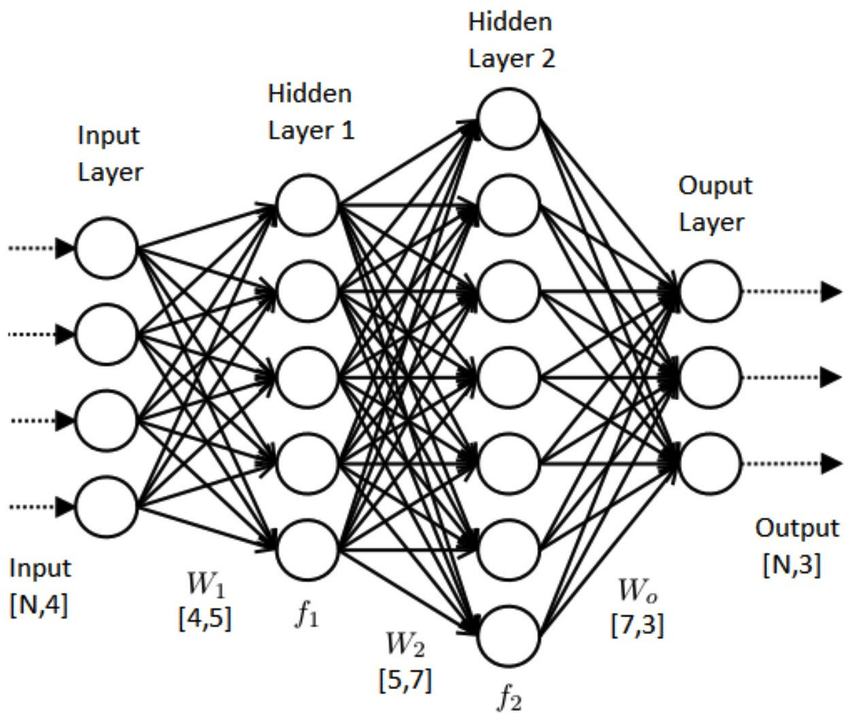
\includegraphics[width=\columnwidth]{mlp}
	\caption{Example of a short caption, which should be centered.}
	\label{fig:mlp}
\end{figure}
\section{Dataset and Processing}
\label{sec:dataset}
\textbf{Pima Indians Diabetes Database}, this dataset originates from the National Institute of Diabetes and Digestive and Kidney Diseases and aims to predict, through diagnostic measurements provided in the dataset, whether or not a patient has diabetes. To create this dataset, specific criteria were applied when selecting instances from a larger database. Notably, all individuals in this dataset are female, at least 21 years of age, and of Pima Indian heritage\cite{smith1988using}.\\
\indent Eight variables were selected as the basis for predicting the occurrence of diabetes within a five-year period in Pima Indian women. These specific variables were chosen because they have been identified as significant risk factors for diabetes in the Pima population or other similar groups, included:
\begin{itemize}
	\item Number of times pregnant
	\item Plasma Glucose Concentration at 2 Hours in an Oral Glucose Tolerance Test (GTT)
	\item Diastolic Blood Pressure (mm Hg)
	\item Triceps Skin Fold Thickness (mm)
	\item 2-Hour Serum Insulin ($\mu$U/ml)
	\item Body Mass Index (Weight in kg / (Height in m)$^2$)
	\item Diabetes Pedigree Function
	\item Age (years)
\end{itemize}\leavevmode\newline
\indent \textbf{Min-Max} and \textbf{Z-score} normalization are applied to features of dataset, and replace $0$ to $-1$ in labels.
\begin{equation*}
	\begin{split}
		Min\_Max:\:\ X^{\prime}_i &= \frac{X_i-\min({X_i})}{\max({X_i})-\min({X_i})} \\
		Z\_score:\: X^{\prime}_i &= \frac{X_i-\overline{X_i}}{\sigma_{X_i}}
	\end{split}
\end{equation*}
where $X^{\prime}_i$ is the nomalized value, $\overline{X}_i$ is the mean value of $i_{th}$ feaure and $\sigma_{X_i}$ is the standard deviation of $i_{th}$ feature.\\
\indent After column-wisely applying Min-Max and Z-score normalizations, we can get the same data values to LibSVM ``scale'' version.

%------------------------------------------------------------------------
\section{Perceptron}
\label{sec:perceptron}
\begin{figure*}[t]
	\centering
	\subfloat[]{\label{fig:neuron}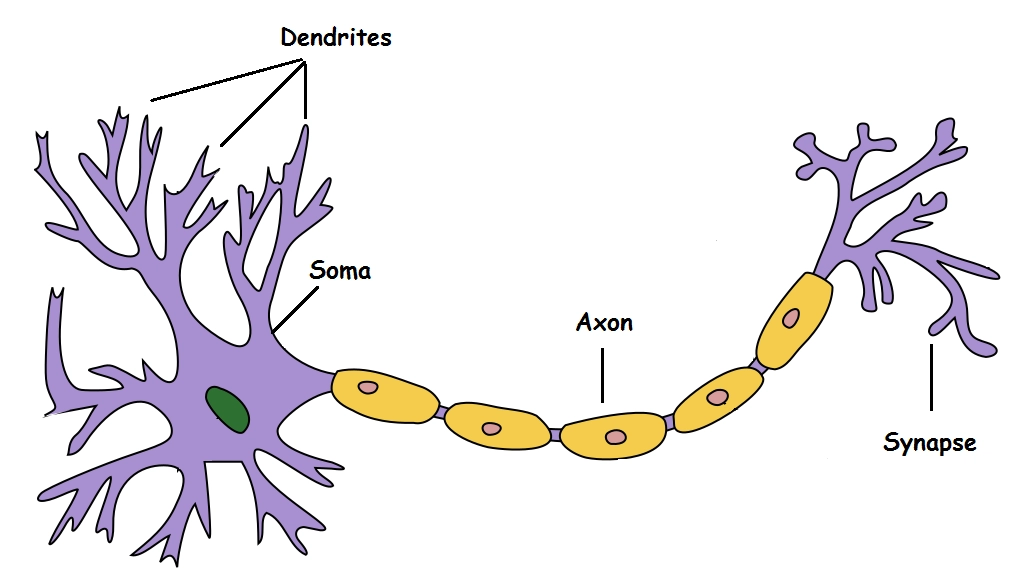
\includegraphics[width=\columnwidth]{neuron}}
	\subfloat[]{\label{fig:mcp}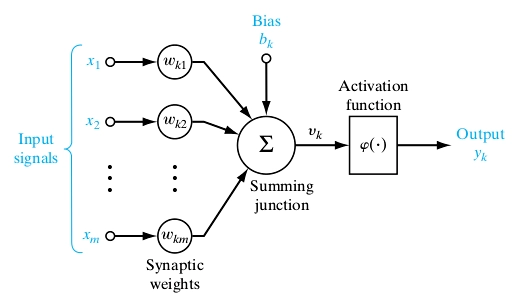
\includegraphics[width=\columnwidth]{mcp}}
	\caption{Example of a short caption, which should be centered.}
	\label{fig:short}
\end{figure*}
Perceptron, proposed by Rosenblatt in 1957, is a simple abstraction of biological neurons and serves as the foundation for neural networks and support vector machines. It is a linear classification model for binary classification, where the input consists of feature vectors for instances, and the output assigns a class label: $+1$ for the positive class and $-1$ for the negative class\cite{rosenblatt1958perceptron}. Perceptron is a discriminative model with the goal of separating positive and negative instances using a separating hyperplane. There is not a unique solution for the perceptron's hyperplane; the perceptron algorithm aims to find one feasible separation. When extended to high-dimensional spaces, it seeks a hyperplane.

\subsection{Linear Separability}
Given a dataset, if there exists a hyperplane, denoted as $S:(wx+b=0)$, that can completely and correctly separate the positive and negative instances of the dataset, such that for $y=+1$ instances, $wx+b>0$, and for $y=-1$ instances, $wx+b<0$, then the dataset is considered linearly separable; otherwise, it is linearly inseparable.

\subsection{Algorithm}
Perceptron can be represented as following:
\begin{equation}
	H(x) = sign(w\cdot x+b)
\end{equation}
\begin{equation}
	sign(x) = \begin{cases}
		+1, x\geq0 \\
		-1, x<0
	\end{cases}
\end{equation}
where $w\in\mathbb{R}^n$ is weight and $b\in\mathbb{R}$ is bias, $w\cdot x$ is the inner product. $sign$ is the signature (activation) function.
\indent First, write down the distance from any point $x_0$ in the input space $\mathbb{R}^n$ to the hyperplane $S$:
\begin{equation}
	\frac{1}{\parallel w \parallel}	\mid w \cdot x_0 + b	\mid
\end{equation}
where $\parallel w \parallel$ is $L2\:norm$ for $w$.\\
\indent For misclassified data $(x_i,y_i)$, the distance from $x_i$ to hyperplane $S$,
\begin{equation}
	-\frac{1}{\parallel w \parallel}y_i(w \cdot x_i + b)
\end{equation}
\indent Therefor, make the set of all misclassified point as $M$, the total distance to hyperplane $S$,
\begin{equation}
	-\frac{1}{\parallel w \parallel}\sum_{x_i \in M}{}y_i(w \cdot x_i + b)
\end{equation}
\indent Ingore $\frac{1}{\parallel w \parallel}$ is the loss function of Perceptron,
\begin{equation}
	L(w,b)=-\sum_{x_i \in M}{}y_i(w \cdot x_i + b)
\end{equation}
\indent Find parameters $w,b$ to minimize the following loss function problem,
\begin{equation}
	\underset{w,b}{min}L(w,b)=-\sum_{x_i \in M}{}y_i(w \cdot x_i + b)
\end{equation}
\indent Perceptron learning algorithm is error-driven and specifically uses stochastic gradient descent\cite{bottou2012stochastic} (SGD).
Initially, it selects an arbitrary hyperplane represented by $w_0,b_0$ and then continuously minimizes the objective function $(7)$ using gradient descent.
During the minimization process, it does not perform gradient descent for all misclassified points in $M$ at once, but instead randomly selects one misclassified point at a time for gradient descent.
The gradient of the loss function $L(w, b)$:
\begin{equation}
	\nabla_w L(w,b)=-\sum_{x_i \in M}y_i x_i
\end{equation}
\begin{equation}
	\nabla_b L(w,b)=-\sum_{x_i \in M}y_i
\end{equation}
\indent Randomly pick a misclassified point $(x_i,y_i) \in M$, update $w,b$:
\begin{equation}
	w \gets w + \eta y_i x_i
\end{equation}
\begin{equation}
	b \gets b + \eta y_i
\end{equation}
where $\eta$ is the learning rate.\\
\indent Through iterations, it is expected that the loss function $L(w, b)$ will continuously decrease, eventually reaching $0$.


\subsection{Implementation}
By creating a class, we can abstract and break Perceptron into different method.
\\
\indent Firstly, we have a method named \textbf{sign}:
\begin{lstlisting}[language={python},numbers=left,tabsize=2]
def sign(self,y):
	return -1 if y < 0 else 1
\end{lstlisting}

And Main function is \textbf{fit} method:
\begin{lstlisting}[language={python},numbers=left,tabsize=2]
def fit(self,x_train,y_train):
	if not self.w:
		self.w = np.zeros(x_train.shape[1])
	for _ in range(self.epoch):
		err=0
		for i in range(len(x_train)):
			xi = x_train[i,:]
			yi = y_train[i]
			yi_hat = self._predict(xi)
			if yi * yi_hat != 1:
				err+=1
				self.w += self.l_rate * yi * xi
				self.b += self.l_rate * yi
		if err == 0:
			break
\end{lstlisting}

Lastly, \textbf{predict} method predicts the whole input dataset:
\begin{lstlisting}[language={python},numbers=left,tabsize=2]
def predict(self,x):
	y_hat = x@self.w.T + self.b
	y_hat = np.where(y_hat<0,-1,1)
	return y_hat
\end{lstlisting}

%------------------------------------------------------------------------
\section{Experiment}
Accuracy refers to the percentage of correct predictions out of the total samples. While accuracy can assess the overall correctness, it may not be a good indicator when dealing with imbalanced datasets.
\begin{equation}
	Accuracy = \frac{TP+TN}{TP+TN+FP+FN}
\end{equation}
Precision represents the probability that a sample predicted as positive is actually positive. Precision measures the accuracy of positive predictions, while accuracy considers both positive and negative predictions.
\begin{equation}
	Precision = \frac{TP}{TP+FP}
\end{equation}
Recall refers to the probability that an actual positive sample is predicted as positive. Higher recall indicates a higher probability of correctly identifying actual positive cases.
\begin{equation}
	Recall = \frac{TP}{TP+FN}
\end{equation}
The F1 score is designed to balance precision and recall, finding a trade-off point between the two.
\begin{equation}
	F1-Score = \frac{2\times Precision\times Recall}{Precision+Recall}
\end{equation}
\\
I use above metrics to do the experiments. Specifically, I also employed K-fold cross-validation, setting K to vary between 3 and 5 to test the performance of different algorithms. The results are as follows:
\begin{tabular}{llrrrr}
	\toprule
	method     & accuracy & precision & recall   & f1       \\
	\midrule
	perceptron & 0.747373 & 0.750533  & 0.747620 & 0.726802 \\
	logistic   & 0.769570 & 0.754407  & 0.722578 & 0.731989 \\
	linear-svm & 0.772176 & 0.759074  & 0.722909 & 0.732924 \\
	rbf-svm    & 0.770894 & 0.758015  & 0.720205 & 0.730358 \\
	mlp        & 0.916667 & 0.928571  & 0.824627 & 0.873518 \\
	\bottomrule
\end{tabular}
From the table, it can be observed that the perceptron has the poorest performance across all metrics, with logistic regression performing slightly better. Linear and kernel-based SVMs exhibit significantly better performance than the perceptron, while MLP outperforms all other methods\dots

\section{Conclusion}
One of the main drawbacks of the perceptron is that it can only address linearly separable problems, meaning it cannot handle situations where there are multiple non-linear decision boundaries within the dataset. Additionally, perceptrons are sensitive to noise and may perform poorly when noise is present or when data is not entirely linearly separable.

%%%%%%%%% REFERENCES
{\small
	\bibliographystyle{ieee_fullname}
	\bibliography{egbib}
}

\end{document}
